%
% exponentialverteilung.tex -- abschnitt ueber Exponentialverteilung in Kapitel 5
%
% (c) 2015 Prof Dr Andreas Mueller, Hochschule Rapperswil
%
\subsection{Exponentialverteilung} \label{section-exponentialverteilung}
\begin{table}
\renewcommand{\arraystretch}{2}
\begin{center}
\begin{tabular}{|l|l|}
\hline
Name&Exponentialverteilung\\
\hline
Dichtefunktion&$\displaystyle ae^{-ax}$,\quad$a>0$\\
Verteilungsfunktion&$1-e^{-ax}$\\
Erwartungswert&$\displaystyle \frac1a$\\
Varianz&$\displaystyle \frac1{a^2}$\\
Median&$\displaystyle \frac1a\log 2$\\[8pt]
$P(|X-E(X)|>\varepsilon)$&
\begin{minipage}{3.7in}
$
\begin{cases}
e^{-a\varepsilon-1}&\qquad\text{für $\varepsilon > \displaystyle\frac1a$}\\
1-e^{a\varepsilon-1}+e^{-a\varepsilon-1}&\qquad\text{für $\varepsilon \le \displaystyle\frac1a$}
\end{cases}
$
\end{minipage}
\\[10pt]
\hline
Anwendungen&\begin{minipage}{3.7in}%
\strut
$\bullet$ Prozess ohne Erinnerungsvermögen\\
$\bullet$ Radioaktivität
\strut
\end{minipage}\\
\hline
\end{tabular}
\end{center}
\caption{Datenblatt der Exponentialverteilung\label{datenblatt:exponentialverteilung}}
\end{table}
\begin{figure}
\begin{center}
%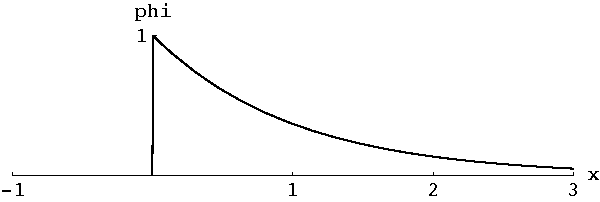
\includegraphics[width=0.8\hsize]{graphics/expphi}
%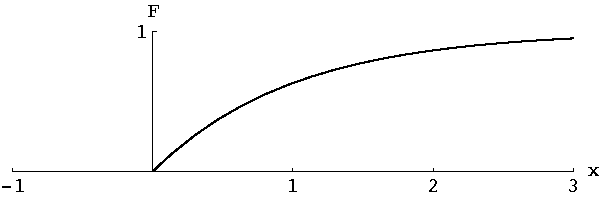
\includegraphics[width=0.8\hsize]{graphics/expF}
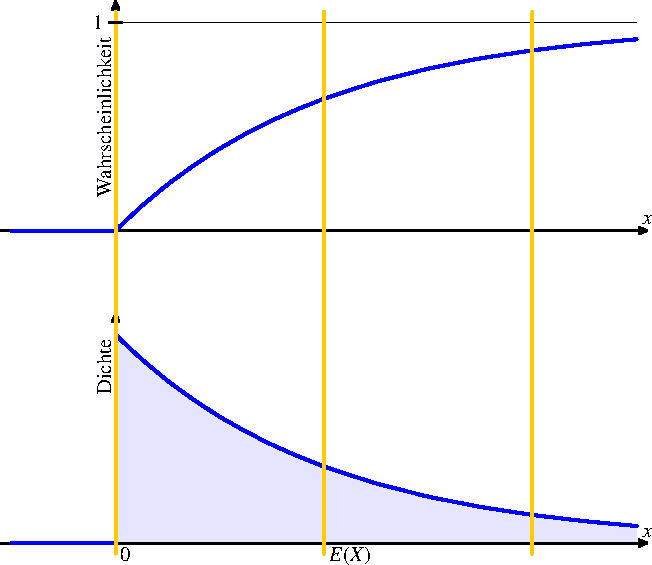
\includegraphics[width=0.8\hsize]{images/verteilungsfunktion-8}
\end{center}
\caption{Verteilungsfunktion (oben) und Dichtefunktion (unten) der
Exponentialverteilung
\label{bildexponentialverteilung}}
\end{figure}
Bei radioaktiven Stoffen und bei gewissen Bauteilen stellt man fest,
dass ihr Zerfall bzw.~ihr Versagen kein Gedächtnis hat.
Die Wahrscheinlichkeit, dass ein Atomkern innerhalb der Zeit $t$ zerfällt,
ist gleich gross wie die Wahrscheinlichkeit, dass er zwischen $t_0$
und $t_0+t$ zerfällt, wenn er bis zur Zeit $t_0$ nicht zerfallen ist.
Auch Bauteile ohne Ermüdungserscheinungen verhalten sich so.

\subsubsection{Verteilungsfunktion und Dichtefunktion}
Etwas formaler sei $X$ eine Zufallsvariable, welche die Zeit angibt, zu der
ein Atomkern zerfällt.
Die ``Gedächtnislosigkeit'' bedeutet, dass die
bedingte Wahrscheinlichkeit für einen Zerfall vor $t_0+t$ unter der
Annahme, dass der Kern bis zur Zeit $t_0$ nicht zerfallen ist, gleich
gross ist wie die Wahrscheinlichkeit eines Zerfalls bis zur Zeit $t$:
\[
P(X \le t) = P(X\le t_0+t\,|\,X > t_0)
\]
Dies ist natürlich gleichbedeutend mit der Wahrscheinlichkeit für
die negierten Ereignisse:
\[
P(X > t) = P(X > t_0+t\,|\,X > t_0)
\]
Aus der Definition~\ref{def-bedingte-wahrscheinlichkeit}
der bedingten Wahrscheinlichkeit folgt
\[
P(X> t_0+t\,|\,X>t_0)=\frac{P(X>t_0+t\wedge X>t_0)}{P(X > t_0)}
=\frac{P(X>t_0+t)}{P(X>t_0)}
\]
Die Bedingung an die Verteilung wird damit zu
\[
P(X>t)P(X>t_0)=P(X>t+t_0).
\]
Schreiben wir jetzt $g(t)=P(X>t)=1-F(t)$, werden die Formeln
etwas übersichtlicher:
\[
g(t)g(t_0)=g(t+t_0).
\]
Zunächst leiten wir nach $t_0$ ab, wir nehmen ja an, dass wir
eine stetige Zufallsvariable haben, und dass die Verteilungsfunktion
differenzierbar sein wird.
Wir erhalten
\[
g(t)g'(t_0)=g'(t+t_0).
\]
Jetzt lassen wir $t_0$ gegen $0$ streben, und bekommen
die Differentialgleichung
\[
g'(t)=g'(0)g(t)
\]
für $g(t)$.
Diese lineare Differentialgleichung erster Ordnung
muss als Lösung eine Exponentialfunktion haben.
Da $F(t)$
monoton wächst, muss $g(t)$ monoton fallen, ausserdem
muss $g(t)$ beschränkt bleiben.
Damit bleibt nur
$g(t)=e^{-at}$ mit einem positiven $a$.

\begin{definition}
Die Wahrscheinlichkeitsverteilung mit Dichtefunktion
\[
\varphi(x)=\begin{cases}
0&\qquad x<0\\
a e^{-a x}&\qquad x\ge 0
\end{cases}
\]
mit $a>0$ heisst Exponentialverteilung.
Ihre Verteilungsfunktion ist
\[
F(x)=\begin{cases}
0&\qquad\text{für $x < 0$}\\
1-e^{-ax}&\qquad\text{für $x\ge 0$}.
\end{cases}
\]
\end{definition}
\index{Exponentialverteilung}
\index{Verteilungsfunktion!Exponentialverteilung}
\index{Wahrscheinlichkeitsdichte!Exponentialverteilung}
Wir sollten noch nachrechnen, dass dies tatsächlich die richtige
Verteilungsfunktion ist.
Zunächst wächst sie tatsächlich monoton,
und auch der Grenzwert für $t\to\infty$ ist wie gewünscht.
Aber
auch die Ableitung ist richtig:
\[
\frac{d}{dt}(1-e^{-at})=ae^{-at}\qquad\text{für}\quad t>0.
\]

\subsubsection{Erwartungswert und Varianz}
\index{Erwartungswert!der Exponentialverteilung}
\index{Exponentialverteilung!Erwartungswert}
\index{Varianz!der Exponentialverteilung}
\index{Exponentialverteilung!Varianz}
\begin{satz}Eine exponentialverteilte Zufallsvariable $X$ mit Parameter
$a$ hat folgenden Erwartungswert und folgende Varianz:
\begin{align*}
E(X)&=\frac1a\\
\operatorname{var}(X)&=\frac1{a^2}
\end{align*}
\end{satz}
\begin{proof}[Beweis]
Zur Berechnung von Erwartungswert und Varianz ist es nützlich die Integrale
$I_n=\int \xi^ne^{-\xi}\,d\xi$
berechnen zu können.
Diese findet man rekursiv durch partielle Integration:
\begin{align*}
I_n&=\int \xi^ne^{-\xi}\,d\xi\\
&=-\xi^ne^{-\xi}+n\int \xi^{n-1}e^{-\xi}\,d\xi\\
&=-\xi^ne^{-\xi}+nI_{n-1}
\end{align*}
Um Erwartungswert und Varianz zu berechnen, verwendet man mit Vorteil die
Variablentransformation $ax=\xi$.
Für den Erwartungswert ergibt sich:
\begin{align*}
E(X)&=\int_0^{\infty}ae^{-ax}x\,dx
=\frac1a\int_0^{\infty}ax e^{-ax}a\,dx
=\frac1a\int_0^{\infty}\xi e^{-\xi}\,d\xi\\
&=\frac1a\left[-\xi e^{-\xi}-e^{-\xi}\right]_0^\infty=\frac1a
\end{align*}
Analog für die Varianz:
\begin{align*}
E(X^2)
&=
\int_0^{\infty}x^2ae^{-ax}\,dx
=\frac1{a^2}\int_0^{\infty}(ax)^2e^{-ax}a\,dx\\
&=\frac1{a^2}\int_0^{\infty}\xi^2e^{-\xi}\,d\xi
=\frac1{a^2}\left[\xi^2e^{-\xi}-2\xi e^{-\xi}+2e^{-\xi}\right]_0^\infty
=\frac2{a^2}
\\
\operatorname{var}(X)
&=E(X^2)-E(X)^2=\frac2{a^2}-\left(\frac1a\right)^2=\frac1{a^2}
\end{align*}
\end{proof}
Die Grösse $\frac1a$ lässt sich also leicht interpretieren: sie ist die
mittlere ``Lebensdauer'', man findet sie oft unter dem Kürzel MTBF für
mean time between failure.
Und $\sqrt{\operatorname{var}(X)}$ 
ist genau gleich gross. 
\index{Mean time between failure}
\index{MTBF}
\subsubsection{Wahrscheinlichkeit grosser Abweichungen}
\begin{figure}
\begin{center}
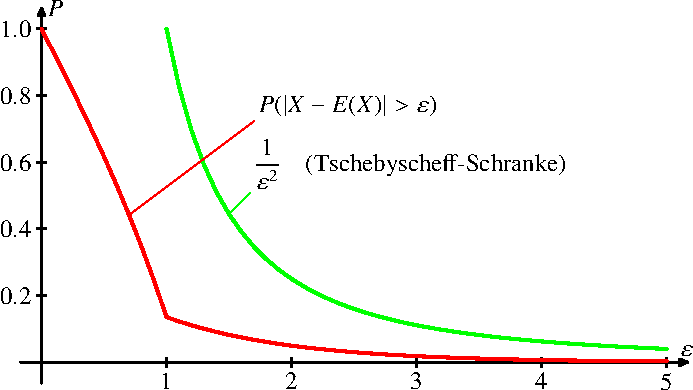
\includegraphics{images/exp-1.pdf}
\end{center}
\caption{Wahrscheinlichkeit für eine grosse Abweichung bei einer
exponentialverteilten Zufallsvariable, oben die durch den Satz von Tschebyscheff
gegebene Schranke (grün), unten die exakte Rechnung mit
Hilfe der Exponentialvereteilung (rot)\label{abweichung-exponential}}
\end{figure}
{
\small
Wir können nun auch die Wahrscheinlichkeit einer grossen Abweichung
berechnen:
\begin{satz} Für eine exponentialverteilte Zufallsvariable mit
Erwartungswert $\frac1a$ ist die Wahrscheinlichkeit einer Abweichung
$\varepsilon$ vom Erwartungswert
\[
P(|X-{\textstyle\frac1a}|>\varepsilon)=
\begin{cases}
e^{-a\varepsilon-1}&\qquad\text{für $\varepsilon > \frac1a$}\\
1-e^{a\varepsilon-1}+e^{-a\varepsilon-1}&\qquad\text{für $\varepsilon \le \frac1a$}
\end{cases}
\]
\end{satz}
\begin{proof}[Beweis]
Die Wahrscheinlichkeit einer grossen Abweichung ist
\begin{align*}
P(|X-{\textstyle\frac1a}|>\varepsilon)
&=1-\int_{\frac1a-\varepsilon}^{\frac1a+\varepsilon}\varphi_a(x)\,dx\\
&=1-\int_{\max(0,\frac1a-\varepsilon)}^{\frac1a+\varepsilon}ae^{-ax}\,dx\\
&=1-\left[-e^{-ax}\right]_{\max(0,\frac1a-\varepsilon)}^{\frac1a+\varepsilon}\\
&=1+e^{-a\varepsilon-1}-e^{-\max(0,1-a\varepsilon)}\\
&=\begin{cases}
e^{-a\varepsilon-1}&\qquad\text{für $\varepsilon > \frac1a$}\\
1-e^{a\varepsilon-1}+e^{-a\varepsilon-1}&\qquad\text{für $\varepsilon \le \frac1a$}
\end{cases}
\end{align*}
\end{proof}
Der Satz von Tschebyscheff setzt diese Wahrscheinlichkeit in Relation
zur Varianz
\[
P(|X-{\textstyle\frac1a}|>\varepsilon)\le
\frac{\operatorname{var}(X)}{\varepsilon^2}=\frac{1}{a^2\varepsilon^2},
\]
selbstverständlich muss diese Ungleichung immer noch erfüllt sein.
Also
\begin{alignat*}{3}
e^{-a\varepsilon-1}&\le&\frac1{a^2\varepsilon^2}&\qquad\text{für $a\varepsilon>1$}\\
1-e^{a\varepsilon-1}+e^{-a\varepsilon-1}&\le&\frac1{a^2\varepsilon^2}&\qquad\text{für $a\varepsilon\le1$}
\end{alignat*}
In allen Ausdrücken kommt immer nur das Produkt $a\varepsilon$ vor,
wir können daher
abkürzend $u=a\varepsilon$ schreiben.
Die zweite Ungleichung wird dann zu
\[
1-\frac{e^{u}-e^{-u}}e=1-\frac{2\sinh u}{e}\le\frac1{u^2}\qquad\text{für $u\le1$}
\]
In diesem Fall ist die rechte Seite mindestens 1,
die Tschebyscheff-Ungleichung wird jetzt völlig nichtssagend, denn 
grösser als 1 kann die Wahrscheinlichkeit für eine Abweichung ohnehin
nicht werden.

Die erste Ungleichung wird zu
\[
e^{-u-1}\le\frac1{u^2}\qquad\text{für $u > 1$}.
\]
Diese Funktion fällt monoton sehr schnell gegen 0, viel schneller
als der Ausdruck $\frac1{u^2}$.
In der Abbildung~\ref{abweichung-exponential}
sieht man beide Schranken, die allgemeine, gegeben durch den
Satz von Tschebyscheff, und die exakte für die Exponentialverteilung.
}

\subsubsection{Anwendung}
Geräte aller Art versuchen, die Lebensdauer dadurch zu erhöhen, dass
kritische Komponenten redundant aufgebaut werden.
Zum Beispiel verwenden Server häufig zwei Disks, deren Daten
gespiegelt sind, so dass der Ausfall eines Disks noch keinen Ausfall
des Gesamtsystems verursacht.
Wir wollen die erwartete Zeit bis zum
Ausfall des Gesamtsystems berechnen, wenn zwei Disks verwendet werden,
deren Zeit bis zum Ausfall exponentialverteilt ist.
Weiter nehmen
wir an, dass die Disks unabhängig voneinander ausfallen.

Sei also $T_i$ die Zeit bis zum Ausfall von Disk $i$, mit
Verteilungsfunktion $F_{T_i}(t)=1-e^{at}$ für $t\ge 0$.
Gesucht
ist die Verteilungsfunktion für die Zeit $T$ bis zum Ausfall
des Gesamtsystems, also die Funktion $F(t)=P(T\le t)$.
Das Gesamtsystem
fällt aus, wenn beide Disks ausgefallen sind, es ist also
\begin{align*}
F(t)
&=P(T\le t)=P(T_1\le t\wedge T_2\le t)\\
&=P(T_1\le t)\cdot P(T_2\le t)
= F_{T_1}(t) F_{T_2}(t)=(1-e^{-at})^2.
\end{align*}
Zur Berechnung des Erwartungswertes von $T$ wird die
Wahrscheinlichkeitsdichte benötigt, also die Ableitung davon:
\begin{equation}
\varphi_{T}(t)=2(1-e^{-at})ae^{-at}.
\label{disks-wdichte}
\end{equation}
Damit wird der Erwartungswert
\begin{align*}
E(T)
&=
\int_{-\infty}^{\infty}t\varphi_T(t)\,dt
=\int_0^\infty 2t(1-e^{-at})ae^{-at}\,dt
\\
&=2\int_0^\infty ate^{-at}\,dt - \int_0^\infty t (2a)e^{-(2a)t}\,dt
=2\cdot\frac1a-\frac1{2a}=\frac{4-1}2\cdot\frac1a=\frac32\cdot\frac1a.
\end{align*}
Durch Redundanz lässt sich die mittlere Zeit bis zu einem Ausfall
also nur um 50\% steigern, die Kosten für das Disksystem werden
aber mehr als verdoppelt.
Abbildung~\ref{graph:disksystem} zeigt, dass die Wahrscheinlichkeit
eines ``frühen'' Ausfalls stark reduziert wird, der eigentliche
Nutzen der Redundanz ist also weniger die Verlängerung der 
Lebensdauer, sondern die Tatsache, dass man darauf verzichten kann,
eine teure Fähigkeit zur sofortigen Reaktion aufzubauen.
\begin{figure}
\centering
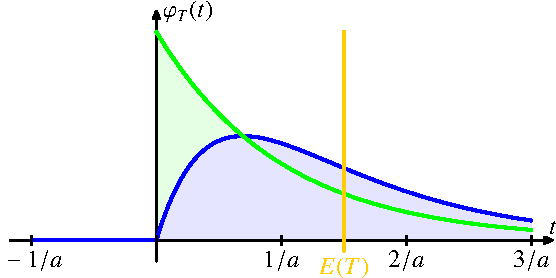
\includegraphics{images/exp-3.pdf}
\caption{Wahrscheinlichkeitsdichte (\ref{disks-wdichte}) 
der Ausfallzeit eines redundanten Disksystems (blau)
im Vergleich zur Verteilung der Ausfallzeit eines einzelnen Disk (grün).
\label{graph:disksystem}}
\end{figure}

